\section{1章 イントロ}
ここでは，ベイズ推測を定義する．
\subsection{ベイズ推測の定義}
\subsubsection{統計的推測の問題設定→機械学習との関連は？}
\({N}\) と \({n}\) を自然数とする．\({N}\) 次元実ユークリッド空間\(\mathbb{R}^N\) 上にn個の点の集合
$$x_1,x_2,...,x_n$$がある場合を考える．言い換えると
$$x_i\in \mathbb{R}^N,\quad (i=1,2,...,n)$$ である．

サンプルをまとめて\({x^n}\) と書く．
つまり
$$x^n = (x_1,x_2,...,x_n) \in \mathbb{R^N} \times \mathbb{R^N} \times \dots \times \mathbb{R^N} = (\mathbb{R^N})^n$$

\noindent\rule{\textwidth}{0.5pt}
ここでサンプルを，確率変数の実現値であることを考える．
この時のサンプル \({x^n}\) の確率密度関数は


で，サンプル \({x_n}\) は上記の確率密度関数で定まる分布に従う確率変数 \({\mathbf{X^N}}\) の実現値と考える．
${q(x)}$を真の分布という．



\begin{quote}
現実には真の分布は不明であって，サンプルだけが与えられることが多い．統計的推測もしくは統計的学習では，与えられた有限n個のサンプルから真の分布を推測することを考える．
統計的推測の手続きによって得られる結果は，確率的に変動するサンプルによるものであるから，これもまた確率的である．
この結果の確率的な挙動を調べる必要がある．（なんで？）
\end{quote}
\subsubsection{サンプルの現れ方に対する平均値}
サンプルを
\subsubsection{ベイズ推測の道具立て：}
\begin{enumerate}
\item 確率モデル
\item 事前分布
\item 逆温度 \({\beta}\) の事後分布
\item 分配関数と周辺尤度
\end{enumerate}
\subsubsection{事後分布による期待値・平均と予測分布}
\subsubsection{ベイズ推測についての著者のまとめ}

\subsection{考察される量について}
\begin{itemize}
\item ベイズ推測のフレームワーク
\begin{itemize}
\item サンプル \({X^N}\)，確率モデル，事前分布 \({\to}\) 予測分布\({p^{*}(x)=p(x|X^N)}\)  を構成する
\item 統計的推測（のプロセスとその結果）は確率的な現象
\end{itemize}
\item 自由エネルギーと汎化誤差が重要な量である
\end{itemize}

\subsubsection{分配関数と自由エネルギー}

\subsubsection{推測と汎化}

\subsubsection{事後分布が計算可能な例}

\begin{enumerate}
\item 指数型分布

\item {\bfseries\sffamily INBOX} 久保川で例題
\end{enumerate}

\subsection{さまざまな統計的推測}


\subsection{事後分布の例（python）}

\if0
読者は「事後分布」という言葉を聞いたときに，どのような形をしていると想像するだろうか。なんとなく「モヤッ」としていて，サンプル数が増えると急峻になってくるものだと想像していないだろうか。ここでは，事後分布の具体的なイメージを得るために事後分布の例をあげてみよう。
\fi


\textbf{例 2} $x \in \mathbb{R}^1$ とし，関数 $\mathcal{N}(x)$ を平均 0 で分散が 1 の正規分布とする。すなわち
\begin{equation}
\mathcal{N}(x) = \frac{1}{\sqrt{2\pi}} \exp\left(-\frac{x^2}{2}\right) \tag{1.26}
\end{equation}
とする。

パラメータ $w = (a,b)$ ($0 \leqq a \leqq 1$, $b \in \mathbb{R}^1$) をもつ確率モデル
\begin{equation}
p(x|w) = (1 - a)\mathcal{N}(x) + a\mathcal{N}(x - b) \tag{1.27}
\end{equation}
を考える．（2 個の正規分布の混合）

\if0
もしも $b$ が原点から十分に離れていれば，例えば $|b| > 3$ 程度に離れていれば，$p(x|w)$ は，二つの区別できる正規分布の和のように見える。
しかしながら $b=0$ のときには，$p(x|w)$ は一つの正規分布を表しているから，$b \approx 0$ では，$p(x|w)$ はほとんど一つの正規分布に見える。
また $a \approx 0$, $a \approx 1$ でも一つの正規分布に見える。
(1.27)式を真の分布として，$a$と$b$の値を変えながら，
このような分布の事後分布を可視化してみる．
\fi



以下では，パラメータの集合が
\begin{equation}
W = \{ (a,b) \ ; \ 0 \leqq a \leqq 1, \ |b| \leqq 5 \} \tag{1.28}
\end{equation}
である場合を考える。また，簡単のために事前分布は場所によらず一定値をとる場合を考える。すなわち
\begin{equation}
\varphi(w) = \frac{1}{10} \tag{1.29}
\end{equation}
とする。この場合，事後分布は尤度関数と同じ形状をしている。また，この例では事後分布 $p(w|X^n)$ を最大にする $w$ が最尤推定量であり，事後確率最大化推定量と同じである。真の分布を $q(x) = p(x|a_0, b_0)$ として
\begin{equation}
(a_0, b_0) \ =\ (0.5, 3.0), \ (0.5, 1.0), \ (0.5, 0.5) \tag{1.30}
\end{equation}
の 3 通りのケースを比較してみよう。$(a_0, b_0)$ を真のパラメータと呼ぶことにする。サンプルの個数は $n=100$ の場合を考える。

\begin{figure}[H]
  \centering
  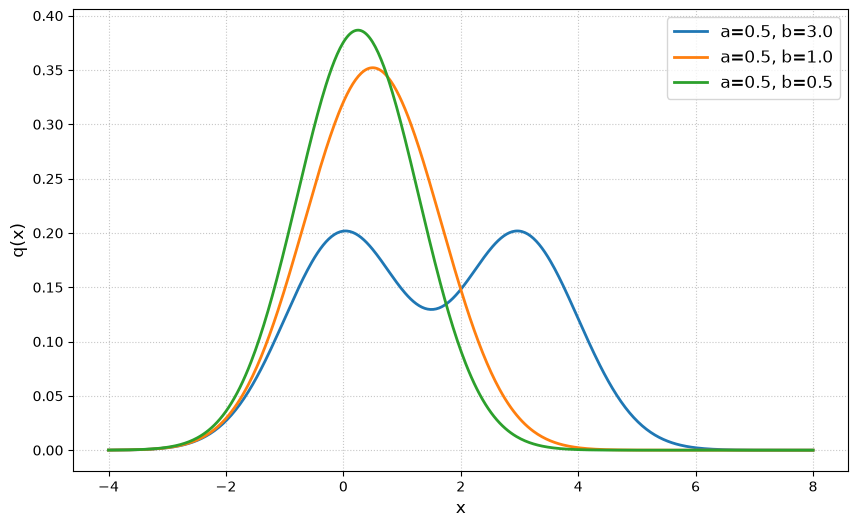
\includegraphics[width=0.5\linewidth]{../../figures/image-3.png}
  \caption{混合正規分布モデル $p(x|w)$ の事後分布の例（$n=100$）}
  \label{fig:posterior-example}
\end{figure}

\subsubsection{ケース(i): $(a_0, b_0) = (0.5, 3.0)$}

二つの確率分布 $\mathcal{N}(x)$ と $\mathcal{N}(x - 3.0)$ は，区別できる程度に離れているので，100 個のデータがあれば真の分布が二つの正規分布の混合であることは明確にわかると思われる。
実際，事後分布を図 1.1 に示す。事後分布は真のパラメータの付近に鋭いピークをもつ分布であり正規分布で近似できそうである。最尤推定量は $(0.47, 3.05)$ であり，真のパラメータ $(0.5, 3.0)$ の近くにある。この場合には事後分布の形状はサンプルの出方にあまり依存しない。事後分布の位置はサンプルの出方によってばらつくが，そのばらつきは小さい。

\subsubsection{ケース(ii): $(a_0, b_0) = (0.5, 1.0)$}

二つの確率分布 $\mathcal{N}(x)$ と $\mathcal{N}(x - 1.0)$ は，重なっている部分が大きく，データが 100 個あっても，真の分布が二つの正規分布の重なりであるのか，一つの正規分布なのかは見分けがつかないかもしれない。
実際，事後分布を図 1.2 に示す。事後分布は真のパラメータの付近からずれて広がっていて正規分布では近似できなさそうである。最尤推定量は $(0.65, 0.55)$ であり，真のパラメータ $(0.5, 1.0)$ からずれている。この場合には同じサンプル数であっても，サンプルの出方により事後分布の位置や形状は変化する。最尤推定量の位置も変化する。

\subsubsection{ケース(iii): $(a_0, b_0) = (0.5, 0.5)$}

二つの確率分布 $\mathcal{N}(x)$ と $\mathcal{N}(x - 0.5)$ は，ほとんど重なっているので，データが 100 個くらいでは，真の分布は一つの確率分布であるように見えるだろう。
実際，事後分布を図 1.3 に示す。事後分布は真のパラメータの近くではなく，$ab \approx 0$ を満たす集合全体のまわりに広がっていて正規分布では近似できない。最尤推定量は $(0.15, 0.71)$ であり，真のパラメータ $(0.5, 0.5)$ とは異なる位置にある。この場合には，事後分布の位置や形状はサンプルの出方により大きく変わる。図 1.3 で示したのは一例にすぎず，サンプルの出方が異なれば，事後分布の形はまったく違ったものになる。最尤推定量もその位置は確率的に大きく変動する。

\begin{figure}[H]
  \centering
  \begin{subfigure}[b]{0.3\linewidth}
    \centering
    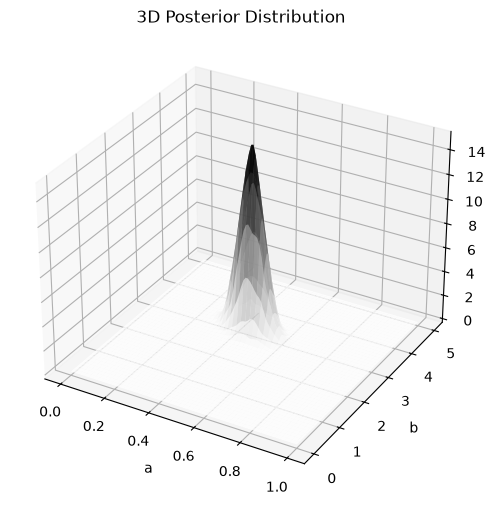
\includegraphics[width=\linewidth]{../../figures/image-4.png}
    \caption{ケース(i): $(a_0,b_0)=(0.5,3.0)$}
    \label{fig:posterior-i}
  \end{subfigure}
  \hfill
  \begin{subfigure}[b]{0.3\linewidth}
    \centering
    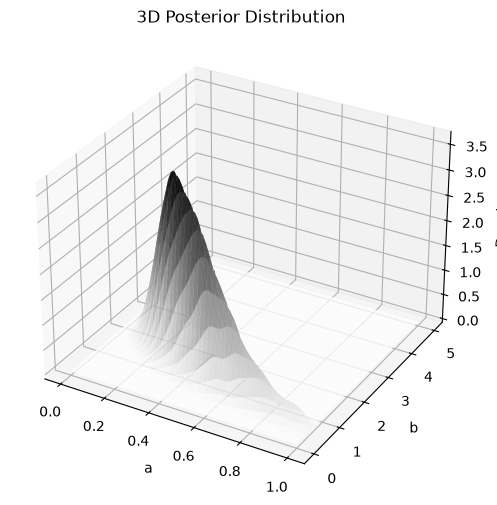
\includegraphics[width=\linewidth]{../../figures/image-5.png}
    \caption{ケース(ii): $(a_0,b_0)=(0.5,1.0)$}
    \label{fig:posterior-ii}
  \end{subfigure}
  \hfill
  \begin{subfigure}[b]{0.3\linewidth}
    \centering
    
\includegraphics[width=\linewidth]{../../figures/image.png}
    \caption{ケース(iii): $(a_0,b_0)=(0.5,0.5)$}
    \label{fig:posterior-iii}
  \end{subfigure}
  \caption{3通りの真のパラメータに対する事後分布（$n=100$）}
  \label{fig:posterior-all}
\end{figure}





\textbf{注意 10} 上記の例はサンプル数が百個の場合のものである。真のパラメータが $(0.5, 0.5)$ の場合にはサンプル数が千個でも，二つの正規分布の区別は付きにくいが，サンプル数が百万個程度あれば，ほぼ区別が付いて事後分布は図 1.1 と同じように真のパラメータの周りに鋭いピークをもつようになる。すなわち事後分布はサンプル数の変化とともにその形を大きく変える。

従来の統計学の理論では，事後分布あるいは尤度関数が図 1.1 のように局所的に鋭いピークをもち正規分布で近似できる場合を想定することが多かった。しかしながら，現実問題では，事後分布が図 1.2，図 1.3 のように大局的な広がりをもつケースがしばしば生じている。また，図 1.1 のように正規分布で近似できる場合を考えると，ベイズ推測も最尤推測も他の推測もほぼ同じ推測精度であるが，図 1.2，図 1.3 のように事後分布が正規分布で近似できない場合には，ベイズ推測が他の方法よりも優れた推測精度をもっていることがわかる。本書では，3 章において事後分布が正規分布で近似できる場合の理論を述べ，4 章で事後分布が大局的な広がりをもつ場合でも扱うことができる理論をつくる。



\subsection{確率モデルの例（久保川）}
\subsection{この本の流れ}
\subsection{一般的注意？？}
\subsection{質問と回答}
\subsection{演習問題}

\noindent\rule{\textwidth}{0.5pt}
